%!TEX root = jir2018aspects.tex
\section{Experimental Method} \label{sec:method}
To address our research questions and examine the hypotheses as outlined in Section~\ref{sec:questions}, we conducted a within-subjects experiment with two factors: system and task. For the system factor, our baseline control system was based on BM25 (no diversification) and a diversified system based on BM25, reranked with xQuAD~\cite{santos2010query_reformulations_diversification}. For the task factor, we used the standard ad-hoc retrieval task and compared against the aspectual retrieval task. This resulted in a $2 \times 2$ factorial design. Each participant therefore completed four different search tasks, one in each of the four conditions (see below). Conditions were assigned using a Latin square rotation to minimise any ordering effects.

%The corpus, topics and system used closely mirror a prior study undertaken by Maxwell et al.~\cite{maxwell2017snippet_length} in which they examined how the length of result summaries affects search behaviour, performance and experience. Summaries of two snippet fragments (roughly equivalent to two lines) resulted in a good tradeoff in terms of examination time and performance. Labelled interface \textbf{\emph{T2}} in their study, we use two snippet fragments in all experimental conditions, as well as the prior nomenclature in the present study. As such, the four experimental conditions we used in this study are listed below.

\begin{itemize}
\item \textbf{(D.As)} A \emph{diversified system}, with an \emph{aspectual retrieval} task.
\item \textbf{(ND.As)} A \emph{non-diversified system}, with an \emph{aspectual retrieval} task.
\item \textbf{(D.Ad)} A \emph{diversified system}, with an \emph{ad-hoc retrieval} task. 
\item \textbf{(ND.As)} A \emph{non-diversified system}, with an \emph{ad-hoc retrieval} task.
\end{itemize}

%Further details of the search systems and tasks are provided in Section~\ref{sec:method:systems}. In this section, we also discuss the corpus and topics that were used (Section~\ref{sec:method:corpus}), how we obtained data for aspectual retrieval (Section~\ref{sec:method:entities}), and the diversification algorithm used (Section~\ref{sec:method:diversification}).

%%%%%%%%
\subsection{Corpus and Search Topics}\label{sec:method:corpus}
For this experiment, we used the \emph{TREC AQUAINT} test collection that contains over one million articles from three newswires, collected over the period $1996$-$2000$. The three newswires were: the \emph{Associated Press (AP)}; the \emph{New York Times (NYT)}; and \emph{Xinhua}.  From the \emph{TREC 2005 Robust Track}~\cite{voorhees2006trec_robust}, we selected five contemporary topics that have been used in prior works~\cite{azzopardi2013query_cost,kelly2009query_suggestion,maxwell2017snippet_length}. These were: ~341 \emph{(Airport Security)}; ~347 \emph{(Wildlife Extinction)}; ~367 \emph{(Piracy)}; ~408 \emph{(Tropical Storms)}; and ~435 \emph{(Curbing Population Growth)}. These topics were chosen based upon evidence from a previous user study with a similar setup, where it was shown that the topics were of similar difficulty and interest~\cite{kelly2009query_suggestion}. Topic~367 was used as a practice topic. The remaining four topics were used as part of the main experimental study.

\subsection{Tasks: Aspectual and Ad-Hoc Retrieval}
Subjects were asked to imagine that they needed to learn about a number of topics on which they were to write a report on. Given a topic, they were further instructed on whether to focus on finding \emph{relevant} articles in the case of ad-hoc retrieval, or \emph{relevant articles that discussed different aspects} of the topic in the case of aspectual retrieval. For example, for the \emph{Airport Security} topic, subjects were required to learn about the efforts taken by international airports to better screen passengers and their carry-on luggage under the ad-hoc retrieval task. For the aspectual retrieval task, they were also asked to find relevant documents that are different and mention \emph{new, previously unseen} airports. Thus, subjects were explicitly instructed to find a number of examples from different airports, as opposed to a similar or the same example based in the same airport multiple times. Subjects were instructed to find and save at least four \emph{useful} documents. Depending upon the task being undertaken, \emph{useful} related to a document being either relevant, or relevant and different.
%From a previous study, we found it took subjects between 5-10 minutes to save 4-8 relevant documents~\anoncite{maxwell2017snippet_length}.

%%%%%%%%
\subsection{Relevance Judgments and Aspects}\label{sec:method:entities}
For each topic, we used the corresponding TREC QRELs from the TREC 2005 Robust Track to provide the relevance judgements for the study. However, to assess how many aspects were retrieved, we needed to commission additional labels, as existing labels were not available for all the selected topics. For each topic, we first examined the topic descriptions to identify what dimensions could be considered aspects of the topic. We noted that for each topic there were at least two ways this could be achieved: entity- or narrative-based. For example, in the topic \emph{Population Growth}, a document could be relevant if it stated the country (entity-based) or measure taken to reduce population growth (narrative-based).
%Thus the country or the measure could be considered different aspects that could be varied, i.e. different countries or different measures or both. 

For this study, it was decided that we should focus on entity-based aspects. This was because ``different narratives'' were subject to greater interpretation than ``different entities''. For each relevant document, two assessors extracted different aspects, and we found that there was substantially higher agreement (95\% vs 67\%) between assessors across the entity based aspects: (341) airports; (347) species; (367) vessels; (408) storms; and  (435) countries; as opposed to the more narrative-based aspects: (341) the security measures taken; (347) the protection and conservation efforts; (367) the acts of piracy; (408) the death and destruction; and (435) the population control methods. Entity-based aspects that we considered for each topic are listed below.

\begin{itemize}
    \item{\textbf{Topic 341 \emph{(Airport Security)}} Different \emph{airports} in which additional security measures were taken, e.g. \emph{John F Kennedy International Airport}, \emph{Boston Logan International Airport}, or \emph{Leonardo Da Vinci International Airport}.}
    \item{\textbf{Topic 347 \emph{(Wildlife Extinction)}} Different \emph{species of endangered animals} under protection by states, e.g. \emph{golden monkey}, \emph{Javan rhino}, or \emph{Manchurian tiger}.}
    \item{\textbf{Topic 367 \emph{(Piracy)}} Different \emph{vessels} that were boarded or hijacked, e.g. \emph{Petro Ranger}, \emph{Achille Lauro}, or \emph{Global Mars}.}
    \item{\textbf{Topic 408 \emph{(Tropical Storms)}} Different \emph{tropical storms} where people were killed or there was major damage, e.g. \emph{Hurricane Mitch}, \emph{Typhoon Linda} or \emph{Tropical Storm Frances}.}
    \item{\textbf{Topic 435 \emph{(Curbing Population Growth)}} Different \emph{countries} where population control methods were employed, e.g. \emph{China}, \emph{India} or \emph{Zimbabwe}.}
\end{itemize}

The total number of aspects identified for each topic were: $14$ for~341, $168$ for~347, $18$ for~367, $43$ for~408, and $26$ for~435. Created judgments were put into the TREC Diversity QREL format, as used by already established evaluation tools that consider aspectual retrieval, such as \texttt{ndeval}\footnote{\url{https://trec.nist.gov/data/web/10/ndeval.c} -- last accessed 2018-12-17.}.\footnote{In the interests of promoting reproducibility and repeatability, the aspectual judgements created as part of this study are available for download at \url{https://git.io/fpAX8}.} %This, in turn, is used as part of the \emph{TREC Novelty and Diversity Tracks} and  the \emph{TREC 2013 Web Track}~\cite{collinsthompson2013trec}.

%%%%%%%%

\begin{figure}[t!]
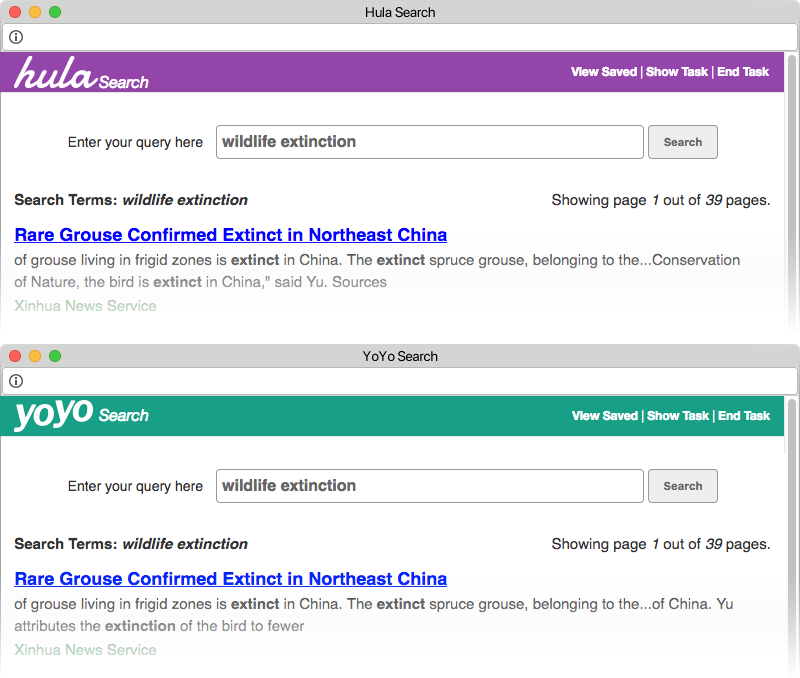
\includegraphics[width=1.0\columnwidth]{figures/interface-both.png}
\caption{The two different search engines and their interfaces, as used in this study. The top screenshot shows \emph{Hula Search} (non-diversified, baseline), with \emph{YoYo Search} (diversified) underneath. Note the different colour schemes that were designed to emphasise the fact that different search systems were being used, without creating too much of a visual distraction.
} 
\label{fig_systems}
\end{figure}

\subsection{Systems: Non-Diversified and Diversified}\label{sec:method:systems}
Two experimental search systems were developed. These were identical except regarding branding/logo and the retrieval algorithm used. First, in terms of branding, we created two fictional search engine names,
\textbf{\emph{Hula Search}} and \textbf{\emph{YoYo Search}}, for which different colour schemes were used. The names were chosen as they were not associated with any major search engine (that we were aware of), nor did they imply that one of the systems performed better than the other. The colour schemes were chosen to provide the greatest difference in visual appearance to those with colourblindness (two variants of colourblindness, \emph{protanopia} and \emph{deuteranopia}, were both considered). This was to ensure that subjects could later on indicate which system that they preferred, etc. Screenshots of the two systems in action are provided in Figure~\ref{fig_systems}. 
Note that a generic \textbf{\emph{NewsSearch}} system -- complete with a blue header -- was used for the practice task. This was done so that subjects could familiarise themselves with how to mark and save documents, and how the search functionality worked.

% \begin{table}[t]
%     \caption{Table illustrating the effects of varying \boldmath{$\lambda$} and diversifying rank cutoff $k$ using \emph{xQuAD}. Values in the table represent the number of new aspects found (aspectual recall) in the top $10$ documents after re-ranking on average, over $715$ queries issued from a prior user study~\anoncite{}. When \boldmath{$\lambda=0.0$}, diversification is not applied -- this configuration therefore enjoys the same performance as our non-diversified system, \textbf{\emph{ND}}, which utilises BM25 (\boldmath{$b=0.75$}).\vspace*{-3mm}}
%     \label{tbl:previous_queries}
%     \renewcommand{\arraystretch}{1.4}
%     \begin{center}
%     \begin{tabulary}{\textwidth}{L{1.2cm}||D{1.0cm}|D{1.0cm}|D{1.0cm}|D{1.0cm}|D{1.0cm}}
%     \hline
    
%     % HEADERS
%     & \multicolumn{5}{c}{\boldmath{$k=$}} \\
    
%     \boldmath{$\lambda=$} & \boldmath{$10$} & \boldmath{$20$} & \boldmath{$30$} \textbf{\emph{(D)}} & \boldmath{$40$} & \boldmath{$50$} \\ \hline\hline
    
%     % VALUES
%     % These results came from sigir-2017-combined.csv -- using an Excel PivotTable. No MATLAB script.
%     \boldmath{$0.0$} \emph{\textbf{(ND)}} & \multicolumn{5}{c}{$3.64$} \\ \hline
%     \boldmath{$0.1$} & $3.64$ & $4.94$ & $5.51$ & $5.95$ & $6.37$ \\ \hline
%     \boldmath{$0.3$} & $6.58$ & $6.58$ & $6.64$ & $6.59$ & $6.59$ \\ \hline
%     \boldmath{$0.5$} & $6.58$ & $6.58$ & $6.58$ & $5.58$ & $6.58$ \\ \hline
%     \boldmath{$0.7$} \emph{\textbf{(D)}} & $6.56$ & $6.56$ & \boldmath{$6.61$} & $6.51$ & $6.60$ \\ \hline
%     \boldmath{$0.9$} & $6.52$ & $6.52$ & $6.61$ & $6.57$ & $6.63$ \\ \hline
%     \boldmath{$1.0$} & $6.63$ & $6.63$ & $6.59$ & $6.61$ & $6.56$ \\ \hline
%     % END
% \end{tabulary}
% \end{center}
% \vspace*{-5mm}
% \end{table}

For the underlying search engine, we used the \emph{Whoosh Information Retrieval (IR)} toolkit.\footnote{Whoosh can be accessed at \texttt{\url{https://pypi.python.org/pypi/Whoosh/}}.} We used BM25 as the retrieval algorithm ($b=0.75$), but with an implicit \texttt{AND}ing of query terms to restrict the set of retrieved documents to only those that contained all query terms provided. This was chosen as most retrieval systems implicitly \texttt{AND} terms together. BM25 served as the baseline control for the non-diversified system condition. For the diversified system condition, we used BM25 to provide the initial ranking and then used xQuAD~\cite{santos2010query_reformulations_diversification} to diversify the ranking. xQuAD has been shown to provide excellent performance for web intent-based diversification. To select the parameters for xQuAD, i.e. $k$, how many documents to re-rank, and $\lambda$ how much focus on diversification, we performed a parameter sweep using a set of training queries from a prior user study~\cite{maxwell2017snippet_length}. We explored a range of $k$ and $\lambda$ values, with $10$--$50$ trialled for $k$, and $0.1$--$1.0$ for $\lambda$. We selected $k=30, \lambda=0.7$ as this configuration provided the best results ($P@10=0.36$, $\alpha DCG@10=0.075$, \emph{aspectual recall (AR)}$@10=6.61$) in terms of performance and efficiency -- i.e. a higher $k$ only slightly increased performance, but took longer to compute.

%% Removed table and revised paragraph below to accommodate missing table.
%Table~\ref{tbl:previous_queries} illustrates the parameter sweep when considering the number of new entities found (aspectual recall) within the top $10$ results, re-ranked after applying xQuAD. Similar conclusions could be reached when examining both $\alpha DCG@10$ (where $\alpha=0.5$) and $P@10$. We found that $k=30$ and $\lambda=0.7$ provided the best results in terms of performance and efficiency -- i.e. a higher $k$ only slightly increased performance, but took longer. 

\subsection{Experimental Procedure}
Subjects were provided with a link to an online experimental system that first presented the information sheet regarding the experiment. This was then followed by the consent form which subjects needed to agree to in order to proceed.\footnote{Ethics approval was sought before the experiment from the Department of Computer and Information Sciences at the University of Strathclyde (ethics approval 622).} Subjects were then asked to fill in a brief demographics survey before undertaking the practice task to familiarise themselves with the interface. Once comfortable with the system, subjects could then proceed to undertake the four search tasks. Depending upon the Latin square rotation, subjects would then be provided with one of the four conditions on one of the four topics. For each task, subjects first completed a pre-task questionnaire. They then moved onto the search task itself. After completion of the task, they were asked to fill in a post-task questionnaire. After completing all four search tasks, subjects were then asked to fill in an exit questionnaire regarding which system they preferred. The experiment would then conclude.

%subjects were provided with a traditional search interface -- complete with query box at the top of the interface. Subjects could pose as few or as many queries as they wished, examine result summaries (as can be seen in Figure~\ref{fig_systems}), and \emph{save} documents they thought were relevant and/or contained new aspects. 10 result summaries were presented per \emph{Search Engine Results Page (SERP)}, \`{a} la the \emph{10 blue links}.


%%%%%%%%
\subsection{Recruitment and Controls}\label{sec:method:subjects}
%%%%%%%%
Subjects for the experiment were recruited via the crowdsourcing platform \emph{Amazon Mechanical Turk (MTurk)}. Previous work has shown that crowdsourced studies provide similar results as traditional lab-based user studies~\cite{kelly2011remote,zuccon2013crowdsourcing}. However, the caveat here is that this is true only if sufficient controls are in place. If not, workers may attempt to game the system and could in theory complete the task poorly~\cite{feild2010turkers}. Therefore, it is important to ensure that quality control mechanisms are in place to mitigate this risk.

First we ensured that the device being used was desktop-based, and the device's screen resolution was at least $1024 \times 768$ or greater in size. As the experiment was conducted via a web browser (i.e. \emph{Chrome}, \emph{Firefox}, \emph{Safari}, \emph{Edge} etc.), we wanted to ensure that only the controls provided by the experimental apparatus were used. The experimental system was therefore launched within a popup window of size $1024 \times 768$. Within the popup, all other browser navigation controls (i.e. back buttons, etc.) were disabled (to the best of our abilities). The experimental system was tested on several major (aforementioned) browsers, across a range of different operating systems. This gave us confidence that similar experiences would be had across different systems.

Based upon the suggestions from prior work~\cite{feild2010turkers,zuccon2013crowdsourcing}, workers were only permitted to begin the experiment on the MTurk platform that:

\begin{itemize}
\item were from the United States;
\item were native English speakers;
\item had a \emph{Human Intelligence Task (HIT)} acceptance rate of at least 95\%; and 
\item had at least 100 HITs approved.
\end{itemize}

Requiring the latter two criteria increased the likelihood of recruiting individuals who wanted to maintain their reputation, and would therefore be more likely to complete the study in a satisfactory manner. 

%Subjects were informed that from prior studies~\anoncite{}, that it would take approximately 7-10 minutes to find at least four relevant documents per task - and the duration of the entire experiment would be approximately 40-50 minutes. 
Subjects were informed that from our pilot study, it would take approximately 7-10 minutes to find at least four relevant documents per task - and the duration of the entire experiment would be approximately 40-50 minutes. Since we did not impose any time constraints on how long they searched for, we imposed an accuracy-based control. We informed participants that their accuracy in identifying relevant material would be examined, and that they should aim to find four useful documents with at least 50\% accuracy (using the TREC relevance judgments as the gold standard). Note that from a previous lab-based study~\cite{maxwell2017snippet_length} for this set of topics, the accuracy of participants was between 25\% and 40\% on average, depending on the topic. While we stipulated a higher accuracy, this was to motivate subjects to work diligently. Since we anticipated the experiment to take just under an hour, participants were compensated with seven dollars (USD).

In all, 64 subjects performed the experiment. However, 13 subjects were omitted either because they failed to complete all search tasks (five subjects were removed), failed to mark at least four documents (two subjects were removed), or spent less than two minutes per task and failed to retrieve any relevant documents (six subjects were removed). 

Of the 51 subjects who successfully completed the experiment, $26$ females and $25$ males participated. The average age of the subjects was $38.66$ years ($min=20$; $max=71$; $stdev=11.43$). $22$ of the subjects reported having a bachelor's degree or higher, with the remaining $29$ possessing an associate degree or lower. All subjects but one expressed \emph{Google} as their everyday search engine of choice. All subjects indicated that they conducted many searches for information via a search engine per week. Nearly three-quarters of the subjects (i.e. 38 subjects) reported using a mouse for the experiment, with the remaining $13$ using some form of trackpad.

%Considering the \todo{$32$} subjects, and the four sessions each subject undertook, this meant a total of \todo{$128$} search sessions were logged.

%We also implemented a series of log post-processing scripts after completion of the study to further identify and capture individuals who did not perform the tasks as instructed. It was from here that we identified the \todo{$20$} subjects that did not complete the search tasks in a satisfactory way -- attaining an accuracy of less than \todo{$50$\%}. These subjects were excluded from the study, reducing the number of subjects reported from \todo{$40$} to \todo{$32$}.



\subsection{Logging and Measures}\label{sec:method:behaviours}
Below we note the measurements taken while participants used the experimental system.
Our system logged a variety of different events associated with querying and assessing. The generated logs permitted us to measure three different aspects of the search user experience, being: \emph{(i)} interaction, \emph{(ii)} performance, and \emph{(iii)} time. 

\paragraph{Interaction Measures} included the number of queries issued by subjects, the number of documents that were examined, the number of different SERPs viewed, and the depths to which subjects clicked on (and hovered over) result summaries. It should be noted that components recorded such as hover depths over result summaries were inferred from the movement of the mouse cursor -- eye-tracking equipment was not used in this study. In prior studies, the position of the mouse cursor on the screen has correlated strongly with the user's gaze on the screen~\cite{chen2001mouse_cursor,smucker2014judging_relevance_movements}.
\vspace*{2mm}

\paragraph{Performance Measures} included the number of documents that were saved by subjects, denoting that they were either relevant (for ad-hoc retrieval), or relevant and contained new information (for aspectual retrieval). From this, we could also break this number down into the number of documents that were saved and TREC relevant -- as well as TREC non-relevant -- and $P@k$ measures at varying depths for the performance of the queries issued by the subjects. Using the diversity QRELs (generated as per the description in Section~\ref{sec:method:entities}), we were able to determine how well the query performed with respect to how many new entities were in the top $k$ results, and the $\alpha$DCG scores for each query. In addition, using the list of saved documents, we could also then identify how many entities that subjects had found, and how many documents contained one or more unseen entities -- both in terms of the context of results of the current query, and the overall search session (over all queries issued).

From the log data, we could also compute additional performance measures such as the accuracy that searchers reached during each session, as well as the \emph{probabilities of interaction.} In the context of this study, accuracy referred to the ratio of documents that were TREC relevant, versus the total numbers of documents saved. For example, if a searcher saved four documents during a search session, with three of them being TREC relevant, the searcher's accuracy was $3/4 = 0.75$. The interaction probabilities that we considered included: the probabilities of clicking on a result summary link ($P(C)$) -- given that it was either TREC relevant ($P(C|R)$) or TREC non-relevant ($P(C|N)$), and the probabilities of marking a document that was clicked ($P(M)$) -- again, given that it was either TREC relevant ($P(M|R)$) or TREC non-relevant ($P(M|N)$).

\paragraph{Time-Based measures} included the time spent issuing queries (from query focus to issuance), the time spent on a SERP -- as well as examining result summaries\footnote{Result summary times were approximated by dividing the total recorded SERP time by the number of snippets hovered over with the mouse cursor. We believe this is a reasonable assumption to make -- network latency issues beyond our control meant that mouse hover events occasionally were delivered at the wrong times, and as such were logged in the incorrect order.} -- and the time spent examining documents. These times then allowed us to compute the total amount of time spent during the search session.

%%%%%%%%
\subsection{User Experience}\label{sec:method:experience}
%%%%%%%%
To capture their perceived experiences, we asked subjects to complete both pre- and post-task surveys for each of the four experimental conditions they undertook.

Pre-task surveys consisted of five questions, each of which was on a seven-point Likert scale ($7$ -- strongly agree to $1$ -- strongly disagree). Subjects were sought for their opinions on their: \emph{(i)} prior knowledge of the topic; \emph{(ii)} the relevancy of the topic to their lives; \emph{(iii)} their desire to learn about the topic; \emph{(iv)} whether they had searched on this topic before; and \emph{(v)} the perceived difficulty to search for information on the topic.

Following the completion of each search task, subjects were provided with a post-task survey, again using a seven-point Likert scale. The survey considered aspects of \emph{(i)} their behaviour, and \emph{(ii)} how they felt the system performed. Considering their behaviours, subjects were asked for their opinions on:
\begin{itemize}
\item how successful they thought they were at completing the task \emph{\textbf{(success)}}; 
\item how quickly they felt they completed the task \emph{\textbf{(subject speed)}}; 
\item whether they issued different queries to explore the topic \emph{\textbf{(queries)}}; 
\item if they only examined a few documents per query \emph{\textbf{(documents)}}; 
\item whether they checked each document carefully before saving \emph{\textbf{(checks)}}; and 
\item whether they saved more documents than was required, with a minimum of four being required \emph{\textbf{(more)}}. 
\end{itemize}
Subjects were also asked for their opinions on: 
\begin{itemize}
\item whether they thought the system helped them complete the task quickly \emph{\textbf{(system speed)}}; 
\item whether they felt the system made it difficult to find useful information \emph{\textbf{(difficulty)}}; 
\item if the system made it easy to complete the task \emph{\textbf{(ease)}}; 
\item if they were happy with how the system performed \emph{\textbf{(happiness)}}; 
\item whether the system was cumbersome or not \emph{\textbf{(cumbersome)}}; and 
\item whether they were confident in the decisions they made \emph{\textbf{(confident)}}. 
\end{itemize}
Upon completion of the experiment, subjects were provided with an exit survey consisting of several questions. Here, we wanted to ascertain which of the two search system offered the best performance, and which one they preferred. 

%We provided a scale from $1$-$6$, from $1$ (definitely \emph{Diversified System Name}) to $3$ (slightly \emph{Diversified System Name}), from $4$ (slightly \emph{Non-Diversified System Name}) to $6$ (definitely \emph{Non-Diversified System Name}). We opted not to include a neutral option to force the subjects into deciding between one of the two systems. We asked subjects: which system was most informative \emph{\textbf{(informative)}}; which was the most unhelpful \emph{\textbf{(unhelpful)}}; which was easiest \emph{\textbf{(easiest)}}; which was the most useful \emph{\textbf{(useful)}}; which system returned the most \emph{relevant} information \emph{\textbf{(rel. preferred)}}; which system returned the most \emph{diverse} information \emph{\textbf{(div. preferred)}}; and which system was preferred overall \emph{\textbf{(preferred)}}.

% From results; moved here to fit in the correct place in the paper.
\begin{table}[t]
    \caption{Query statistics and performance measures across both of the experimental systems trialled, \textbf{\textit{ND}} (Non-Diversified) and \textbf{\textit{D}} (Diversified). Note the significant differences between the diversity-centric measures, \boldmath{$\alpha DCG$} (where \boldmath{$\alpha=0.5$}) and Aspectual Recall (\boldmath{$AspR.$}), highlighting that the diversification algorithm did indeed provide a more diverse set of results to the subjects.}
    \label{tbl_queryperf_2018}
    \renewcommand{\arraystretch}{1.5}
    \begin{center}
    \begin{tabulary}{\textwidth}{L{0.2cm}L{5.75cm}|D{2.1cm}|D{2.1cm}}
    %\begin{tabulary}{\textwidth}{cc|c|c}
    
    \hline
    
    % OUTPUT FROM script
    &  & \textbf{\emph{ND}} & \textbf{\emph{D}} \\ \hline\hline
    & \textbf{\emph{Queries Issued}} & $718$ & $555$ \\ \hline
    & \textbf{\emph{Terms per Query}} & $3.59$ & $3.80$ \\ \hline
    & \textbf{\emph{Unique Terms}} & $345$ & $292$ \\ \hline\hline
     
    \multirow{2}{*}{\rotatebox{90}{\hspace*{-1mm}\small{\boldmath{$Prec.$}}}} & \boldmath{$P@5$} & $0.25\pm 0.01$* & $0.29\pm 0.01$*  \\ \cline{2-4}
    & \boldmath{$P@10$} & $0.22\pm 0.01$ & $0.24\pm 0.01$  \\ \hline\hline
      
    \multirow{2}{*}{\rotatebox{90}{\hspace*{-1mm}\small{\boldmath{$\alpha DCG$}}}} & \boldmath{$\alpha DCG@5$} & $0.02\pm 0.00$* & $0.04\pm 0.00$* \\ \cline{2-4}
    & \boldmath{$\alpha DCG@10$} & $0.03\pm 0.00$* & $0.04\pm 0.00$* \\ \hline\hline
       
    \multirow{2}{*}{\rotatebox{90}{\hspace*{-1mm}\small{\boldmath{$AspR.$}}}} & \boldmath{$AspR.@5$} & $1.40\pm 0.11$* & $3.39\pm 0.21$*  \\ \cline{2-4}
    & \boldmath{$AspR.@10$} & $2.11\pm 0.14$* & $4.07\pm 0.24$*  \\ \hline    
    \end{tabulary}
    \vspace*{-4mm}
    \end{center}
\end{table}

